
\section{Processi organizzativi}

\subsection{Processo di coordinamento}
\subsubsection{Comunicazioni}
\paragraph{Responsabilità}
Al fine di ottenere comunicazioni chiare e coincise il \textit{\RdP} deve gestirle in modo strutturato, utilizzando la forma che meglio si adatta alla situazione.
Le comunicazioni possono essere interne o esterne al \textit{team\ped{G}}.
\paragraph{Comunicazioni interne}
\subparagraph{Descrizione}
In funzione della tipologia di comunicazione interna si deve decidere quale modalità di presentazione delle informazioni deve essere adottata: formale o informale; scritta o orale.
In funzione di questi due criteri, le principali forme di comunicazione che vengono adottate sono:
\begin{itemize}
\item
\textbf{Comunicazione formale scritta}: questa modalità di comunicazione viene utilizzata quando si vuole che esse assumano un carattere di ufficialità e per tutte quelle comunicazioni che sono di fondamentale importanza per la corretta gestione del progetto;
\item
\textbf{Comunicazione verbale formale}: le comunicazioni a carattere divulgativo o di presentazione;
\item
\textbf{Comunicazione informale scritta}: quella scambiata tra due o più membri del \textit{team\ped{G}} senza carattere di ufficialità ma utile a chiarire o puntualizzare alcuni aspetti del progetto;
\item
\textbf{Comunicazione informale orale}: questo tipo di comunicazione avviene in tutti quei contesti in cui vengono scambiate opinioni e informazioni sulla attività di progetto.
\end{itemize}

Per ogni tipologia di comunicazione si è deciso di utilizzare i seguenti strumenti:
\begin{itemize}
\item
\textit{\PdP}, convocazioni di riunione e verbali di riunione per le comunicazioni formali scritte;
\item
Presentazioni e discorsi per le comunicazioni verbali formali;
\item
E-mail, \textit{instant messaging\ped{G}} e \textit{web storage\ped{G}} per le comunicazioni informali scritte;
\item
Riunioni e conversazioni per le comunicazioni informali orali.
\end{itemize}

Il \textit{team\ped{G}} ritiene fondamentale la comunicazione interna per:
\begin{itemize}
\item
Trasmettere informazioni sulle esigenze tecniche ed operative;
\item
Informare i membri del \textit{team\ped{G}} su principi, politiche, strategie, obiettivi che regolano e definiscono il comportamento dell'organizzazione;
\item
Motivare i membri del \textit{team\ped{G}}, realmente e concretamente.
\end{itemize}


\paragraph{Comunicazioni esterne}
\subparagraph{Descrizione}
Il \textit{team\ped{G}} ha ritenuto idoneo creare una casella di posta elettronica per le comunicazioni esterne, denominata:

\begin{center} \url{thefellowshipofthecode@gmail.com} \end{center}

La gestione delle relazioni con i proponenti e con i committenti è affidata al \textit{\RdP}, il quale è tenuto, quando ritiene necessario, aggiornare i membri del 	\textit{team\ped{G}} riguardo le informazioni ottenute.


\subsubsection{Riunioni}

\paragraph{Finalità}
Le riunioni sono vitali per gestire un progetto. Vanno gestite con attenzione per non sprecare tempo, per aumentare la produttività e la motivazione del \textit{team\ped{G}} e per risolvere eventuali problemi. Una riunione è produttiva quando genera nuove idee o consolida una iniziativa, senza trasformarsi in un boomerang.
Una riunione ben organizzata, oltre a perseguire uno specifico obiettivo, motiva le persone generando fiducia ed armonia tra i membri del gruppo.

\paragraph{Riunioni interne}
\subparagraph{Ruoli}
\subsubparagraph{Moderatore}
Il \textsl{\RdP} ha il compito di convocare le riunioni interne, ovvero gli incontri generali a cui partecipano tutti i membri.
Ad ogni riunione il \textsl{\RdP} verificherà il numero dei presenti per decidere se confermare o meno l'incontro.
Il \textsl{\RdP} ha l'obbligo di rendere le riunioni produttive, a tal fine
esso deve fungere da guida nella discussione degli argomenti, essere fonte di ispirazione e avere l'autorità per seguire l'ordine del giorno e per trovare il consenso sulle decisioni da prendere.
Il \textsl{\RdP}, essendo il coordinatore della riunione, è tenuto ad avere un atteggiamento:
\begin{itemize}
\item
\textbf{Flessibile}: saper essere fermo quando occorre, senza dimostrarsi prepotente e meno severo a seconda delle situazioni;
\item
\textbf{Autorevole}: avere sempre il controllo della situazione e il rispetto dei partecipanti;
\item
\textbf{Assertivo}: mantenere un'adeguata comunicazione e saper ascoltare chi parla. Il maggior contributo deve essere quello di introdurre gli argomenti, fare domande per stimolare la discussione e trarre le conclusioni.
\end{itemize}
\subsubparagraph{Segretario}
Il \textit{Segretario} ha il compito di tenere la minuta dell'incontro, controllare che siano stati discussi tutti i punti previsti dalla riunione e di redigere
il verbale. Alla fine di ogni riunione, il \textit{Segretario} deve inviare ai partecipanti copia del verbale dell'incontro, un rendiconto delle decisioni prese e delle responsabilità assunte e le raccomandazioni in previsione del prossimo incontro. Ciò consentirà di mantenere informato anche chi non ha potuto partecipare al meeting.
\subsubparagraph{Partecipanti}
Ad ogni incontro i membri del gruppo devono sentirsi responsabilizzati ad arrivare preparati e mantenere un comportamento consono volto al miglioramento degli obiettivi di essa.
Ogni membro del gruppo può richiedere al \textit{\RdP} di indire una riunione interna, in surplus a quella settimanale, motivando la richiesta. Spetterà al responsabile del progetto decidere se approvare o meno la richiesta.
\subparagraph{Descrizione}
La convocazione delle riunioni avranno cadenza settimanale, il \textit{\RdP} invierà una email ad ogni membro del gruppo informandolo della riunione.
Ogni membro del gruppo è tenuto ad inviare una mail di risposta confermando la presenza o motivando l'assenza.
Affinché una riunione abbia validità, è necessario che siano presenti almeno la metà più uno dei membri del \textit{team\ped{G}}, in caso contrario la riunione sarà annullata e spostata a data da destinarsi.

Le riunioni interne sono ritenute uno strumento fondamentale per:
\begin{itemize}
\item
Scambiare delle informazioni e relazioni tra i membri;
\item
Riconoscere i meriti ai migliori membri;
\item
Rafforzare lo spirito di appartenenza all'organizzazione da parte di tutto il gruppo;
\item
Stimolare e motivare a fare sempre meglio.
\end{itemize}

Le riunioni, generalmente, si dividono in quattro tipi:
\begin{itemize}
\item
Riunioni per informare;
\item
Riunioni per valutare;
\item
Riunioni per decidere;
\item
Riunioni per progettare.
\end{itemize}

Le decisioni dovranno riguardare:
\begin{itemize}
\item
La definizione degli obiettivi da raggiungere;
\item
La designazione dei responsabili;
\item
La scelta dei mezzi;
\item
La determinazione dei tempi di esecuzione;
\item
Il fissare la data di una nuova ed eventuale riunione.
\end{itemize}

Importante è la gestione del dopo riunione, attraverso la compilazione di un verbale che metta a conoscenza tutti i membri del \textit{team\ped{G}} delle decisioni prese.

\paragraph{Riunioni esterne}
\subparagraph{Descrizione}
Le riunioni con proponente/i o con committente/i sono ritenute di fondamentale importanza per instaurare un rapporto di fiducia tra le parti, condividere gli obiettivi e i bisogni.
L'organizzazione delle riunioni esterne sarà affidata al \textit{\RdP}, o in caso straordinario a qualunque membro del gruppo, qualora quest'ultimo abbia ricevuto il consenso da parte del \textit{\RdP}.
Al termine di ogni riunione, il \textit{\RdP} o un suo delegato dovrà verbalizzare quanto emerso ed eventuali richieste di cambiamenti riguardanti elementi che possono avere degli impatti negativi sulla realizzazione del progetto.

\subsection{Processo di pianificazione}

\subsubsection{Descrizione}
Durante l'intero sviluppo del progetto didattico ogni componente del gruppo
dovrà obbligatoriamente cimentarsi in tutti i ruoli elencati di seguito. \\
Inoltre non potrà mai accadere che un membro del gruppo risulti redattore e verificatore di un medesimo documento.
In questo modo si tende ad evitare il conflitto di interessi che potrebbe sorgere se la responsabilità della stesura e della verifica di un documento fosse affidata ad un'unica persona.
Un membro può inoltre ricoprire più ruoli contemporaneamente.

\paragraph{\RdP}
Il \textit{\RdP} è colui che detiene la responsabilità del
lavoro svolto dall'intero \textit{team\ped{G}}. Rappresenta inoltre colui che mantiene i
contatti diretti presso il fornitore e il cliente, ovvero gli enti esterni. Più
in dettaglio, ha responsabilità su:
\begin{itemize}
  \item Pianificazione, coordinamento e controllo generale delle attività;
  \item Gestione delle risorse;
  \item Analisi e gestione dei rischi;
  \item Gestione e approvazione della documentazione;
  \item Contatti con gli enti esterni.
\end{itemize}
Il \textit{\RdP} redige l'\textit{organigramma\ped{G}}, si assicura che
tutte le attività vengano svolte seguendo rigorosamente le \textit{\NdP}, si
assicura che vengano rispettati i ruoli assegnati nel \textit{\PdP} e che non si
presentino conflitti di interesse tra redattori e verificatori. Ha inoltre
l'incarico di creare, assegnare ad ogni membro e gestire i singoli task. Redige
il \textit{\PdP} e collabora alla stesura del \textit{\PdQ}. Il \textit{\RdP} è
l'unica persona in grado di approvare in modo definitivo un documento.

\paragraph{Amministratore}
L'\textit{\Amm} è il responsabile di tutto ciò che riguarda l'ambiente di
lavoro. Più in dettaglio, egli si occupa di:
\begin{itemize}
  \item Controllo dell'ambiente di lavoro;
  \item Gestione del versionamento della documentazione tramite l'uso di
  database;
  \item Controllo delle versioni e delle configurazioni del prodotto;
  \item Risoluzione dei problemi legati alla gestione dei processi.
\end{itemize}
L'\textit{\Amm} redige le \textit{\NdP} e collabora alla stesura del
\textit{\PdP}.

\paragraph{Progettista}
Il \textit{\Prog} è il responsabile di tutto ciò che riguarda la progettazione.
Più in dettaglio, egli si occupa di:
\begin{itemize}
  \item Produrre una soluzione attuabile, robusta e semplice entro i limiti di
  tempo stabiliti;
  \item Effettuare scelte progettuali volte a garantire la manutenibilità e la
  modularità del prodotto software.
\end{itemize}
Il \textit{\Prog} redige la \textit{\ST}, la \textit{\DDP} e la parte
programmatica del \textit{\PdQ}.

\paragraph{Analista}
L'\textit{\Ana} si occupa di tutto ciò che riguarda l'analisi del problema da
affrontare. Le mansioni principali sono quelle di:
\begin{itemize}
  \item Studiare a fondo e capire le problematiche del prodotto da realizzare;
  \item Produrre una specifica di progetto compresibile per il
  \textit{proponente}, per il \textit{committente} e per il
  \textit{Progettista}.
\end{itemize}
L'\textit{\Ana} redige lo \textit{\SdF}, l'\textit{\AdR} e parte del
\textit{\PdQ}.

\paragraph{Verificatore}
Il \textit{\Ver} è responsabile di tutto ciò che riguarda l'attività di verifica.
Effettua la verifica dei documenti utilizzando gli strumenti e i metodi proposti nel
\textit{\PdQ} e seguendo rigorosamente quanto descritto nelle \textit{\NdP}.
Egli ha il compito di garantire la conformità rispetto le \textit{\NdP} dei documenti da lui verificati.
Si occupa di redigere la sezione del \textit{\PdQ} che illustra l'esito delle
verifiche effettuate sui documenti.

\paragraph{Programmatore}
Il \textit{\Progr} si occuperà di implementare le soluzioni del \textit{\Prog}, è quindi
responsabile dell'attività di codifica. In dettaglio, i suoi compiti sono:
\begin{itemize}
  \item implementare le soluzioni descritte dal \textit{\Prog} in maniera
  rigorosa;
  \item Scrivere il codice rispettando le convenzioni prese nel presente
  documento;
  \item Implementare i test per il codice scritto da utilizzare per l'attività
  di verifica.
\end{itemize}
Il \textit{\Progr} redige il \textit{\MU} e produce la documentazione del codice.

\subsection{Strumenti}

\subsubsection{Google Drive}
\textit{Google Drive\ped{G}} è un servizio di storage online utilizzato dal
\textit{team\ped{G}} per condividere file e documenti che non necessitano di tracciamento.
\textit{Google Drive\ped{G}} consente anche il lavoro concorrente su uno stesso
file.
\subsubsection{GitHub}
Gli strumenti software per il controllo versione sono ritenuti molto spesso necessari per la maggior parte dei progetti di sviluppo software.
Per questo motivo, il \textit{team\ped{G}} ha deciso di creare un \textit{repository\ped{G}}, ospitato all'interno di un server, per gestire la continua evoluzione dei documenti digitali come il codice sorgente del software, la documentazione testuale e altre informazioni importanti.
Il software di versionamento scelto è \textit{Git\ped{G}} perchè presenta molti più aspetti positivi rispetto ai \textit{repository\ped{G}} centralizzati. \textit{Git\ped{G}} permette di lavorare anche in assenza di connettività con il server centrale. I membri del \textit{team\ped{G}} possono lavorare sulla propria copia locale del \textit{repository\ped{G}} e rendere pubbliche le modifiche caricandole nel \textit{repository\ped{G}} centrale. Questo approccio risulta molto semplice e veloce per poter collaborare con i membri del \textit{team\ped{G}} simultaneamente.
Inoltre online è possibile reperire moltissima documentazione a riguardo per un rapido apprendimento. Il servizio scelto per il mantenimento dei dai è \textit{GitHub\ped{G}}. \\La struttura base del \textit{repository\ped{G}}:
\begin{itemize}
  \item
	RR;
	\begin{itemize}
		\item
			Interni;
		\item
			Esterni.
	\end{itemize}
  \item
    RQ;
  \item
    RP;
  \item
  	RA;
  \item
  	Template.
\end{itemize}

\subsubsection{Gestione delle attività del progetto}
Per gestire nella maniera più opportuna la divisione del lavoro, si è scelto di
utilizzare il sistema di pianificazione delle attività \textit{Zoho\ped{G}}.

\subsubsection{Task management}
Vengono creati dal \textit{\RdP} e sono assegnati a due singoli membri del gruppo,
il primo in qualità di redattore e il secondo in qualità di \textit{\Ver}.
Per una gestione più chiara di questa divisione delle attività, sono stati creati su \textit{Zoho\ped{G}}
due insiemi di \textit{task\ped{G}} per ogni documento, definiti:
\begin{itemize}
  \item \textit{Nome del documento};
  \item \textit{Nome del documento - da verificare}.
\end{itemize}
Una volta che il proprietario ritiene il suo \textit{task\ped{G}} completato, deve spostarlo
nella relativa sezione \textit{da verificare} in modo tale che il verificatore
interessato possa controllarlo e segnarlo come completato, se risulta idoneo.

\paragraph{Creazione di un elenco di task}
Un elenco di \textit{task\ped{G}} rappresenta l'insieme dei \textit{task\ped{G}} necessari per la realizzazione di un intero documento.
Per la creazione di un nuovo insieme di \textit{task\ped{G}} bisogna seguire le seguenti istruzioni:
\begin{enumerate}
   \item Dalla HomePage di \textit{Zoho\ped{G}} selezionare il progetto interessato (\progetto);
  \item Selezionare la voce \textbf{Compiti e Pietre miliari} dal menù laterale;
   \item Selezionare la voce \textbf{Nuovo elenco di compiti} e compilare l'elenco di \textit{task\ped{G}} nel
  seguente modo:
  \begin{itemize}
    \item \textbf{Elenco dei compiti:} assegnare il nome del documento che si
    vuole rappresentare;
    \item \textbf{Pietra miliare collegata:} selezionare a quale pietra miliare si
    vuole collegare la realizzazione di questo insieme di \textit{task\ped{G}}. Corrispondono alla
    versione finale del documento.
  \end{itemize}
\end{enumerate}
\paragraph{Creazione di un task}
Per la creazione di un nuovo singolo \textit{task\ped{G}} bisogna seguire le seguenti
istruzioni:
\begin{enumerate}
  \item Dalla HomePage di \textit{Zoho\ped{G}} selezionare il progetto interessato (\progetto);
  \item Selezionare la voce \textbf{Compiti e pietre miliari} dal menù laterale;
  \item Selezionare la voce \textbf{Nuovo compito} e compilare il \textit{task\ped{G}} nel
  seguente modo:
    \begin{itemize}
      \item \textbf{Nome task:} assegnare un nome identificativo al \textit{task\ped{G}} seguito dalla \textit{milestone\ped{G}} corrispondente;
      \item \textbf{Aggiungi descrizione:} inserire una descrizione breve ma
      concisa del \textit{task\ped{G}}, deve avere la seguente forma:
        \begin{itemize}
          \item Redattore: nome del redattore;
          \item Verificatore: nome del verificatore.
        \end{itemize}
      \item \textbf{Elenco dei compiti:} selezionare uno degli elenchi di
      \textit{task\ped{G}}, creati precedentemente, che hanno come fine ultimo la realizzazione di un
      documento;
      \item \textbf{Chi è il responsabile?:} inserire l'intestatario del \textit{task\ped{G}}
      come primo utente, nel secondo invece inserire il verificatore assegnato;
      \item \textbf{Data di conclusione:} Inserire la data ultima per il
      completamento del \textit{task\ped{G}};
     \item \textbf{Priorità:} inserire, opzionalmente, una priorità al \textit{task\ped{G}}.
    \end{itemize}
\end{enumerate}


\paragraph{Modifica di un task}
Per modificare un \textit{task\ped{G}} seguire le seguenti istruzioni:
\begin{itemize}
  \item Selezionare il \textit{task\ped{G}} da modificare;
  \item Dalla pagina proposta selezionare il campo che si vuole modificare;
  \item Completata la modifica premere il pulsante \textbf{Invio}.
\end{itemize}

\paragraph{Completamento di un task}
Dopo che il verificatore ha appurato che il \textit{task\ped{G}} soddisfa i requisiti, e quindi è stato redatto secondo le
\textit{\NdP}, può procedere con il suo completamento seguendo le seguenti istruzioni:
\begin{itemize}
  \item Selezionare il \textit{task\ped{G}} da segnare come completato;
  \item Nella parte inferiore della pagina proposta selezionare la voce \textbf{Contrassegna come completato}.
\end{itemize}
Dopo questa operazione, il \textit{task\ped{G}} viene spostato automaticamente nella lista dei \textit{task\ped{G}} completati. Da qui, in
casi eccezionali, può essere rispostato nei \textit{task\ped{G}} \textit{da verificare}. Questi casi eccezionali possono essere:
\begin{itemize}
  \item Il \textit{\RdP} non ha approvato il documento e quindi deve essere
  rivisto;
  \item Il \textit{\Ver}, dopo un secondo controllo sui \textit{task\ped{G}} a lui assegnati,
  può accorgersi di errori e/o incompletezze. Deve quindi essere rivisto.
\end{itemize}
\newpage
\section{Meccanismi di controllo e di rendicontazione}
	\subsection{Meccanismi di controllo} Sono stati adottati dei meccanismi, nell'ambiente creato, per:
	\begin{itemize}
		\item Controllare l'andamento delle attività;
		\item Permettere un aggiornamento facilitato della pianificazione;
		\item Rendicontare le ore di lavoro spese nelle varie attività.
	\end{itemize}
	\subsection{Controllo ritardi di attività}  Per mantenere il controllo sull'andamento generale si è scelto di adottare dei metodi grafici.
		\subsubsection{Dettaglio attività} Il sistema di ticketing adottato permette di visualizzare in modo dinamico il \textit{diagramma di  Gantt\ped{G}} delle attività. Viene visualizzato:
		\begin{itemize}
			\item La percentuale di completamento di ognuna di esse;
			\item Le attività in ritardo;
			\item Le attività concluse.
		\end{itemize}
		\begin{center}
			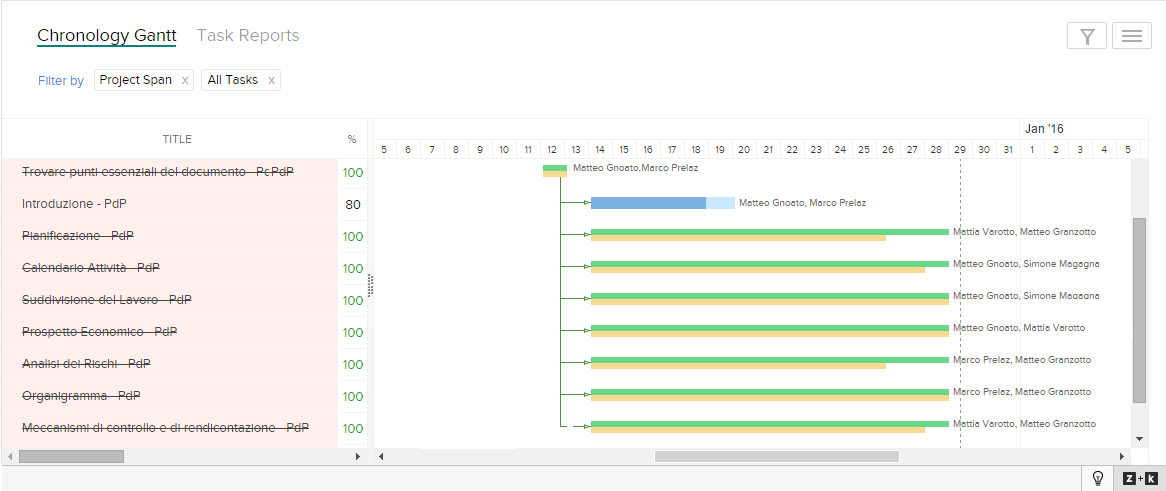
\includegraphics[keepaspectratio = true, width=16cm]{immagini/PdP_ZohoGantt.png}
		\end{center}
		\begin{figure}[h]
			\caption{\textit{Diagramma di Gantt\ped{G}} prodotto dal sistema di ticketing adottato.}\label{etichetta}
		\end{figure}
		\subsubsection{Fasi processi}
		Combinando i dati del sistema di ticketing in un grafico ad area in pila per visualizzare il numero di ticket aperti in un particolare stato del \textit{ciclo di Deming\ped{G}}, è immediato visualizzare in quali stati si trovino le attività.
		\subsubsection{Controllo date} Per ottimizzare la pianificazione e tenerla in costante aggiornamento si utilizzano dei calendari a disposizione del gruppo.
		\subsubsection{Calendario attività}
		Il sistema di ticketing adottato genera automaticamente un calendario in cui vengono indicate inizio e fine delle varie attività.
		\subsubsection{Calendario risorse} Il calendario a disposizione del gruppo utilizzato per gestire il personale in base agli impegni dei vari componenti.
		\subsubsection{Controllo metriche di progetto} L'introduzione delle metriche consente di quantificare nel modo più obiettivo possibile le performance del gruppo nello svolgimento del progetto attraverso la misurazione dell'insieme di indicatori che ne fanno parte. Tipicamente uno degli usi più importanti delle metriche è quello di misurare l'avanzamento del progetto a fronte del piano. Il loro utilizzo consente di: 
		\begin{itemize}
			\item Identificare i problemi di costo/schedulazione prima che diventino criticità;
			\item Aiutare il \textit{team\ped{G}} a focalizzarsi sul completamento delle proprie attività.
		\end{itemize}
		In particolare le metriche \textit{Budget Variance\ped{G}}(BV) e \textit{Schedule Variance\ped{G}}(SV) permettono rispettivamente di:
		\begin{itemize}
			\item Indicare se si è speso di più o di meno rispetto a quanto previsto;
			\item Indicare se si è in linea, in anticipo o in ritardo rispetto alla schedulazione delle	attività di progetto pianificate nella \textit{baseline\ped{G}}. 
		\end{itemize}
		I valori aggiornati di tali metriche sono riportati nel \textit{\PdQ}.
	\subsection{Meccanismi di rendicontazione} Il sistema di ticketing adottato mette a disposizione la rendicontazione delle ore di lavoro. Tale sistema permette di visualizzare le ore di lavoro in base all'attività svolta.
\subsection{Lista di controllo}
Durante l'applicazione della tecnica del \textit{Walkthrough\ped{G}} ai documenti sono stati riportati
più frequentemente i seguenti errori:
\begin{itemize}
  \item\textbf{Norme stilistiche}:
  \begin{itemize}
    \item La prima parola di una voce dell'elenco puntato non inizia con una lettera maiuscola;
    \item La voce dell'elenco puntato termina con un punto anziché con un punto e virgola o viceversa;
    \item I due punti in grassetto;
    \item Errori di battitura;
    \item Comando nuova riga non deve essere utilizzato per le descrizioni di descrizione ed utilizzo;
    \item Le immagini e il testo devono stare dentro il range della pagina;
    \item Dopo il nome di un metodo e di un parametro non ci vanno i :;
    \item Parametri di un metodo non devono avere l'accessibilità;
    \item Gli array vanno indicati così: Array<Tipo>;
    \item Tutti i metodi hanno tipo di ritorno, se qualcosa non ritorna niente è void;
    \item I costruttori non hanno tipo di ritorno. 
     
  \end{itemize}

  \item\textbf{Italiano}:
  \begin{itemize}
    \item Maiuscole usate impropriamente.
    
  \end{itemize}

  \item\textbf{\LaTeX}:
  \begin{itemize}
  \item Mancato utilizzo dei comandi \LaTeX{} personalizzati;
  \item Scambiato il comando \verb|\textit{...}| con \verb|\textbf{...}|;
  
  \end{itemize}
  
  \item\textbf{Casi d'Uso}:
  \begin{itemize}
	\item Mancato rispetto del template stabilito per i punti trattati nei casi d'uso.
  \end{itemize}

	\item\textbf{Glossario}:
	\begin{itemize}
		\item Sono stati evidenziati dei termini che non andavano nel \textit{\G{}};
		\item Non sono stati evidenziati dei termini che sono presenti nel \textit{\G{}}.
	\end{itemize}

\end{itemize}
